% ============================================================
%  Ask What Matters — Technical Slide Deck
%  2026 Wharton Hack-AI-thon | Expedia Group
% ============================================================
\documentclass[aspectratio=169,10pt]{beamer}

\usepackage[T1]{fontenc}
\usepackage[utf8]{inputenc}
\usepackage{lmodern}
\usepackage{microtype}
\usepackage{amsmath}
\usepackage{amssymb}
\usepackage{listings}
\usepackage{xcolor}
\usepackage{tikz}

% ── Theme ────────────────────────────────────────────────────
\usetheme{default}

\setbeamerfont{frametitle}{size=\large, series=\bfseries}

\setbeamertemplate{navigation symbols}{}
\setbeamertemplate{footline}{%
  \begin{beamercolorbox}[wd=\paperwidth,ht=2ex,dp=1ex]{normal text}%
    \hfill\tiny\insertframenumber\hspace{1em}
  \end{beamercolorbox}%
}
\setbeamertemplate{frametitle}{%
  \vspace{0.4em}%
  \hyphenpenalty=10000\exhyphenpenalty=10000%
  \insertframetitle\par%
  \vspace{-0.2em}%
  \rule{\textwidth}{0.4pt}\par%
  \vspace{0.15em}%
}

% ── Code style ───────────────────────────────────────────────
\lstset{
  basicstyle=\ttfamily\scriptsize,
  keywordstyle=\bfseries,
  frame=single,
  framerule=0.3pt,
  breaklines=true,
  tabsize=2,
  showstringspaces=false,
  language=Python,
  xleftmargin=0.5em,
  xrightmargin=0.5em,
  aboveskip=0.3em,
  belowskip=0.3em,
}

\newcommand{\arrow}{$\rightarrow$}
\newcommand{\shead}[1]{\smallskip\textbf{#1}\par\smallskip}

% ── Title ────────────────────────────────────────────────────
\title{\textbf{Ask What Matters}}
\subtitle{Adaptive AI for Smarter Travel Reviews\\[0.3em]
  \small 2026 Wharton Hack-AI-thon\quad|\quad Expedia Group}
\author{Bailey McIntosh}
\date{April 2026}

\begin{document}

% ── TITLE ────────────────────────────────────────────────────
\begin{frame}[plain]
  \titlepage
\end{frame}


% ════════════════════════════════════════════════════
\section{Problem \& Thesis}
% ════════════════════════════════════════════════════

\begin{frame}{The Core Problem: The Reviewer Side}
\begin{itemize}
  \item Reviewers produce \textbf{generic content} — staff friendliness,
        cleanliness — regardless of what prospective guests actually need
  \item Surveys and follow-up forms see low compliance; reviewers resist
        structured prompts that feel like extra work
  \item Post-stay motivation is low: the reviewer has no stake in downstream
        traveler decisions
  \item A 2023 Phocuswright study found $>60\%$ of OTA reviews fail to mention
        at least one category the booking traveler later cited as decision-relevant
\end{itemize}

\bigskip
\textbf{Core tension:}
The people who \textit{write} reviews optimize for expressing their experience.
The people who \textit{read} reviews optimize for resolving specific uncertainties.
These objectives rarely align by accident.
\end{frame}


\begin{frame}{The Core Problem: The Prospective Guest Side}
\begin{itemize}
  \item Guests must infer property attributes from a corpus of \textit{incidentally}
        written reviews — effectively a \textbf{missing-data inference problem}
  \item High-variance topics (noise levels, breakfast quality) are especially
        underserved: few reviewers volunteer them, yet they drive booking decisions
  \item Review volume inflates confidence without improving \textbf{topical coverage}:
        $n=200$ reviews that all mention location add no information about the pool
  \item Existing systems (Expedia, TripAdvisor, Booking.com) surface category averages
        but do not \textit{direct} reviewer attention toward information gaps
\end{itemize}

\bigskip
\alert{Key insight:} More reviews do not solve the problem.
\textit{Better-directed} reviews do.
Can we guide reviewers toward the topics that matter most to future guests,
without adding friction or perceived burden?
\end{frame}


\begin{frame}{Thesis: Demand-Driven Reviewer Nudging}

\textit{If we surface, at the moment of review composition, the precise topics
that prospective guests have signaled uncertainty about, reviewers will include
that information — not because they are compelled, but because they are shown
its value.}

\bigskip
\textbf{Two signals combined:}
\begin{itemize}
  \item \textbf{Supply signal} — gap analysis over the existing review corpus:
        which topics are under-documented or contested?
  \item \textbf{Demand signal} — prospective guest questions (SNSAS):
        which topics are travelers actively asking about?
\end{itemize}

\bigskip
\textbf{Behavioral framing:}
Reviewers resist being \textit{told} what to write.
Framing the nudge as ``here is what others are still unsure about'' converts
review-writing into an act of social contribution, triggering prosocial
motivation rather than compliance friction.
\end{frame}


\begin{frame}{Why Existing Approaches Fall Short}
\begin{columns}[T]
\column{0.48\textwidth}
\textbf{Where current approaches fail}
\begin{itemize}
  \item Category rating forms force discrete input and too many controls
  \item Review template prompts add perceived burden and reduce flow
  \item NLP post-hoc extraction only analyzes what was already written
  \item Static FAQ / Q\&A content stays isolated from the review corpus
  \item Sentiment summaries compress tone, not information coverage
\end{itemize}

\column{0.48\textwidth}
\textbf{How our system departs}
\begin{itemize}
  \item We surface topics without forcing structured answers
  \item The nudge is non-blocking and visible at a glance
  \item We intervene \textit{before} composition, not after submission
  \item Demand signals reshape future review content at the source
  \item We distinguish missing information from already-covered topics
\end{itemize}
\end{columns}

\medskip
\textbf{Key departure:} Every existing approach is reactive — it acts on reviews
after they are written. Our system acts \textit{during} composition, when the
reviewer can still be guided.
\end{frame}


% ════════════════════════════════════════════════════
\section{System Architecture}
% ════════════════════════════════════════════════════

\begin{frame}{System Architecture Overview}
\begin{columns}[T]
\column{0.48\textwidth}
\textbf{Core pipeline}
\begin{enumerate}
  \item Load review corpus, property descriptions, and traveler demand data
  \item Score coverage gaps with a 4-signal analyzer
  \item Generate a compact ``Travelers still want to know'' panel
  \item Track topic coverage live while the user writes
\end{enumerate}

\medskip
\textbf{Feedback loop}
\begin{itemize}
  \item Browse page collects traveler questions (SNSAS)
  \item Question classifier maps them into topic buckets
  \item Demand scores feed back into future gap prioritization
\end{itemize}

\column{0.48\textwidth}
\textbf{System components}
\begin{itemize}
  \item \textbf{Data:} reviews, property descriptions, traveler\_questions.csv
  \item \textbf{Scoring:} embeddings + VADER + LLM + traveler demand
  \item \textbf{Generation:} \texttt{gpt-4o-mini} for nudge intro text
  \item \textbf{Interface:} Streamlit — review, browse, and thank-you states
\end{itemize}

\medskip
\textbf{Stack}\\
\small
Streamlit for hosting, OpenAI for generation and embeddings,
VADER for fast local sentiment.
All expensive steps are cached with \texttt{@st.cache\_data}.
\end{columns}
\end{frame}


\begin{frame}{Data Model: Review Corpus \& Time Weighting}
\begin{columns}[T]
\column{0.52\textwidth}
\textbf{Reviews\_PROC.csv}
\begin{itemize}
  \item 13 properties, $\sim$1{,}600 total reviews
  \item Key fields: \texttt{eg\_property\_id}, \texttt{review\_text},
        \texttt{acquisition\_date}, \texttt{rating} (JSON dict)
  \item At load time: \texttt{rating} parsed to structured dict;
        \texttt{acquisition\_date} coerced to \texttt{datetime64}
  \item \textbf{Time-decay weighting} per property:
        \[w_i = \exp\!\Bigl(-\tfrac{\ln 2}{\tau}\cdot d_i\Bigr)\]
        where $d_i$ = days since review, $\tau = 180$ days (half-life)
  \item Top-$N$ weighted reviews ($N=40$) selected for embedding
\end{itemize}

\column{0.44\textwidth}
\textbf{Why time-decay weighting?}\\[0.3em]
\small
Older reviews describe a hotel that may no longer exist: new ownership,
renovations, staff turnover. Exponential decay with a 180-day half-life
ensures recent guest experiences dominate gap detection.

\medskip
\textbf{Top-$N=40$ selection:}
Full embedding of all 1{,}600 reviews is expensive.
Selecting the top-40 by weight is $4\times$ cheaper while retaining
the most informative recent signal.
\end{columns}
\end{frame}


\begin{frame}{Data Model: Topic Taxonomy \& Traveler Questions}
\begin{columns}[T]
\column{0.52\textwidth}
\textbf{Topic Taxonomy — 15 fixed categories}
\begin{itemize}
  \item \textbf{10 universal:} Location, Room Quality, Service,
        Atmosphere, Bathroom, Sleep Quality, Noise, Value,
        Cleanliness, Check-in
  \item \textbf{5 conditional:} Food, Breakfast, Pool/Facilities,
        WiFi, Parking — gated on property amenity data
  \item Each topic has a label, keyword list, icon, and a
        \textbf{dense anchor phrase} for embedding comparison
  \item Anchor phrases beat short labels: \textit{``hotel noise
        levels quiet loud soundproofing street traffic walls rooms
        disturb sleep''} embeds more specifically than
        \textit{``Noise Levels''}
\end{itemize}

\column{0.44\textwidth}
\textbf{traveler\_questions.csv}\\[0.3em]
\small
Fields: \texttt{eg\_property\_id}, \texttt{question},
\texttt{topic}, \texttt{timestamp}, \texttt{source}

\medskip
Intentionally \textbf{never cached} — always read fresh so a question
submitted in one browser tab is immediately visible to a reviewer in
another tab.

\medskip
\textbf{Why anchor phrases?}
Short labels embed near many irrelevant concepts.
Rich descriptive phrases occupy a more specific region of the
latent space, improving cosine similarity precision.
\end{columns}
\end{frame}


% ════════════════════════════════════════════════════
\section{Feature 1: TWTK Algorithm}
% ════════════════════════════════════════════════════

\begin{frame}{TWTK Algorithm: Four-Signal Overview}

\texttt{analyze\_property(property\_id, demand=())} returns up to 3
gap topics per property. Four independent signals feed a single scorer.

\medskip
\begin{columns}[T]
\column{0.48\textwidth}
\textbf{The four signals}
\begin{enumerate}
  \item \textbf{Embedding coverage} — what fraction of recent reviews
        substantively discuss each topic?
  \item \textbf{VADER sentiment variance} — are guest opinions on a
        topic split (contested)?
  \item \textbf{LLM unique topics} — what property-specific gaps does
        GPT-4o-mini find that the taxonomy misses?
  \item \textbf{SNSAS demand} — which topics are prospective guests
        actively asking about?
\end{enumerate}

\column{0.48\textwidth}
\textbf{Gap types produced}
\begin{itemize}
  \item \textbf{gap} — coverage below threshold ($< 0.15$)
  \item \textbf{contested} — high sentiment variance
        ($\sigma_{\text{VADER}} \geq 0.38$)
  \item \textbf{demand} — well-covered but travelers are asking
  \item \textbf{unique} — LLM-discovered, outside taxonomy
\end{itemize}

\medskip
\textbf{Filtering}\\
\small
A topic surfaces only if:
$\text{cov} < 0.15$ \textbf{or} $\sigma \geq 0.38$ \textbf{or} $d > 0$
\end{columns}
\end{frame}


\begin{frame}{Signal 1: Semantic Coverage via Embeddings}
\begin{columns}[T]
\column{0.52\textwidth}
\textbf{Algorithm}
\begin{enumerate}
  \item Embed top-$N$ weighted reviews with
        \texttt{text-embedding-3-small} (batch call).
        Result: $R \in \mathbb{R}^{N \times 1536}$, row-normalised.
  \item Embed one \textbf{anchor phrase} per topic (cached globally).
        Result: $\mathbf{a}_l \in \mathbb{R}^{1536}$ per label $l$.
  \item Cosine similarity: $\text{sim}_{il} = \hat{r}_i \cdot \hat{a}_l$.
        Review is \textit{on-topic} iff $\text{sim}_{il} \geq \theta_r = 0.40$.
  \item \textbf{Coverage} = weighted fraction of on-topic reviews:
        \[\text{cov}_l = \frac{\sum_{i:\,\text{sim}_{il}\geq\theta_r} w_i}{\sum_i w_i}\]
  \item Flag as \textit{gap} if $\text{cov}_l < \theta_g = 0.15$.
\end{enumerate}

\column{0.44\textwidth}
\textbf{Design decisions}\\[0.3em]
\small
\textbf{Why review-level here, sentence-level in real-time?}
Per-sentence embedding gives live keypress feedback.
Whole-review embedding in corpus analysis is sufficient
and $10\times$ cheaper.

\medskip
\textbf{Threshold $\theta_r = 0.40$:}
Below this, reviews mention a word adjacent to the topic but do not
discuss it substantively.
Tuned empirically on the 13-property corpus.

\medskip
\textbf{Why anchor phrases, not topic labels?}
Short labels embed near many irrelevant concepts.
Rich phrases occupy a more specific latent region.
\end{columns}
\end{frame}


\begin{frame}[fragile]{Signal 2: VADER Sentiment Consensus}
\begin{columns}[T]
\column{0.52\textwidth}
\textbf{Algorithm}
\begin{enumerate}
  \item Collect on-topic texts $\mathcal{T}_l$; require
        $|\mathcal{T}_l| \geq 4$.
  \item Compute VADER compound score $s_t \in [-1,1]$ for each
        $t \in \mathcal{T}_l$.
  \item Std dev of scores: $\sigma_l = \text{std}(\{s_t\})$.
        Flag as \textbf{contested} if $\sigma_l \geq \theta_c = 0.38$.
\end{enumerate}

\begin{lstlisting}
sentiments = [
    vader.polarity_scores(t)["compound"]
    for t in on_topic_texts
]
if np.std(sentiments) >= CONTESTED_STD:
    is_contested = True
\end{lstlisting}

\column{0.44\textwidth}
\textbf{Design rationale}\\[0.3em]
\small
\textbf{What ``contested'' signals:}
High variance means some guests rated the topic highly, others poorly.
Their concrete experience helps future guests resolve genuine uncertainty.

\medskip
\textbf{Why VADER over a transformer?}
VADER is rule-based and runs in $<1$ms per text.
At 40 reviews $\times$ 15 topics, a neural model would add
${\sim}3$--$5$ seconds per page load.

\medskip
\textbf{$\theta_c = 0.38$ rationale:}
VADER compound scores cluster tightly for homogeneous corpora
($\sigma \approx 0.1$--$0.2$).
A threshold of $0.38$ fires only on genuine bimodality.
\end{columns}
\end{frame}


\begin{frame}{Signal 3: LLM-Discovered Unique Topics}
\begin{columns}[T]
\column{0.52\textwidth}
\textbf{\texttt{discover\_unique\_topics(property\_id)}}\\[0.3em]
\small
\textbf{Motivation:} The 15-topic taxonomy covers hotel universals.
Each property has idiosyncratic gaps — a safari lodge's
\textit{``Big Five sighting probability''}, a mountain hotel's
\textit{``Snow conditions''} — that no fixed taxonomy can anticipate.

\medskip
\textbf{Prompt inputs:} property name, city, description (600 chars),
amenities (300 chars), 12 most recent review texts.

\medskip
\textbf{Task:} Ask GPT-4o-mini what a prospective guest would be
\textit{genuinely uncertain} about that the reviews fail to answer.
Exclude generic topics; return \texttt{[]} if no genuine gaps exist.

\medskip
\textbf{Output:} JSON array, up to 2 items:
\texttt{[\{"label": "...", "icon": "emoji"\}]}

\column{0.44\textwidth}
\textbf{Integration \& tradeoffs}\\[0.3em]
\small
Unique topics are appended with a fixed score of $0.2$ and are
\textbf{not} boosted by demand (SNSAS maps to the fixed 15-label
taxonomy; unique topics are outside the anchor dictionary).

\medskip
One GPT-4o-mini call per property, cached.
Temperature $= 0.3$ for reproducible but not mechanical output.
Cap at 2 items — beyond 2, the LLM tends to hallucinate relevance.

\medskip
\textbf{Guard rails:}
\begin{itemize}
  \item ``Do NOT suggest generic topics''
  \item ``Return \texttt{[]} if no genuine gaps exist''
  \item JSON-only output requirement
\end{itemize}
\end{columns}
\end{frame}


\begin{frame}[fragile]{Signal 4 \& Scoring: Demand Weighting}
\begin{columns}[T]
\column{0.52\textwidth}
\textbf{Demand signal derivation}\\[0.3em]
\small
Normalise SNSAS question counts to $[0,1]$:
\[d_l = \frac{c_l}{\max_j c_j}\]
where $c_l$ = count of user questions mapped to topic $l$.
The most-asked topic always scores $d_l = 1.0$.

\medskip
\textbf{Cache-busting:} demand is passed as a sorted hashable tuple,
forcing re-computation of \texttt{analyze\_property} whenever
the question set changes:
\begin{lstlisting}
demand_tuple = tuple(sorted(
    get_demand_scores(pid, questions_df).items()
))
gaps = analyze_property(pid, demand=demand_tuple)
\end{lstlisting}

\column{0.44\textwidth}
\textbf{Final scoring formula}\\[0.3em]
\small
\[
\text{score}_l =
\text{base}_l \times (1 + \beta_d \cdot d_l)
\]

\textbf{Base scores by gap type:}
\[
\text{base}_l = \begin{cases}
1 - \text{cov}_l & \text{gap (cov} < 0.15) \\[3pt]
0.5(1 - \text{cov}_l) & \text{contested} \\[3pt]
0.4\,d_l & \text{demand-only}
\end{cases}
\]

$\beta_d = 3.0$: at this value, a single SNSAS question roughly
doubles the score of a mid-strength gap topic.

\medskip
Top-3 by score are returned.
LLM-unique topics are appended at a fixed score of $0.2$,
not competing with formula-scored topics.
\end{columns}
\end{frame}


\begin{frame}{Real-Time Reviewer Feedback: \texttt{covered\_topics()}}
\begin{columns}[T]
\column{0.52\textwidth}
\textbf{Algorithm}
\begin{enumerate}
  \item Split the in-progress review on \texttt{[.!?]+} into sentences
        of length $> 8$ chars.
  \item For each sentence, call \texttt{embed\_sentence()} — cached
        by content, so unchanged sentences incur no API cost.
  \item Compute cosine similarity against each gap topic's anchor.
  \item A topic is \textit{covered} if any sentence
        scores $\geq \theta_r = 0.40$.
  \item Update the TWTK panel live: covered topics show a green
        checkmark; footer switches to \textit{``You've covered
        everything''} when all gaps are addressed.
\end{enumerate}

\column{0.44\textwidth}
\textbf{Latency management}\\[0.3em]
\small
\textbf{Why sentence-level at keypress?}
Whole-review re-embedding on each keypress would lag.
Per-sentence caching means only new or modified sentences
trigger API calls.

\medskip
\textbf{Post-submission insights:}
After posting, \texttt{extract\_insights()} calls GPT-4o-mini
to produce one factual sentence per covered topic, shown on the
thank-you page to reinforce the reviewer's contribution.

\medskip
\textit{Example:} ``Bathroom: Shower has strong water pressure
and reliable hot water throughout the day.''
\end{columns}
\end{frame}


% ════════════════════════════════════════════════════
\section{Feature 2: Browse \& SNSAS}
% ════════════════════════════════════════════════════

\begin{frame}{Feature 2: Browse Page \& SNSAS}
\begin{columns}[T]
\column{0.50\textwidth}
\textbf{Browse page}
\begin{itemize}
  \item Top-10 most recent reviews per property, sorted descending
  \item Long reviews ($>300$ chars) collapsed with
        \textit{Read more $\downarrow$} toggle
  \item Expand/collapse state keyed per review index,
        persisted in Streamlit session state
\end{itemize}

\medskip
\textbf{SNSAS form} (Still Not Sure About Something)
\begin{itemize}
  \item Free-text question input
  \item On submit: classify \arrow\ append to CSV \arrow\ clear text area
        (via counter-keyed widget key)
  \item Wipe button resets demo data (\texttt{source="user"} rows only)
\end{itemize}

\column{0.46\textwidth}
\textbf{\texttt{classify\_question\_topic(question)}}\\[0.3em]
\small
Maps free-text questions to one of 15 canonical labels:
\begin{enumerate}
  \item Embed question: $\mathbf{q} \in \mathbb{R}^{1536}$
  \item Find highest-similarity anchor:
        $\hat{l} = \arg\max_l\; \hat{\mathbf{q}} \cdot \hat{\mathbf{a}}_l$
  \item Return that label
\end{enumerate}

No threshold cutoff — every question maps somewhere.
Edge cases degrade gracefully to the nearest category.

\medskip
Cached by question string, so repeated demo submissions are free.
\end{columns}
\end{frame}


\begin{frame}{The Demand Feedback Loop: End to End}

\begin{enumerate}
  \item A prospective guest browses a property page and submits a question
  \item \texttt{classify\_question\_topic()} maps it to a topic label
  \item The question is appended to \texttt{traveler\_questions.csv}
  \item \texttt{get\_demand\_scores()} converts topic counts to
        normalised demand $d_l$
  \item The next reviewer's TWTK panel is re-ranked using that demand signal
  \item New reviews then address the topics travelers are actively asking about
\end{enumerate}

\bigskip
\begin{columns}[T]
\column{0.48\textwidth}
\textbf{Temporal dynamics}\\[0.2em]
\small
Questions accumulate over time. The demand signal strengthens as more guests
ask the same thing, creating urgency proportional to collective uncertainty
rather than individual preference.

\column{0.48\textwidth}
\textbf{Live during the demo}\\[0.2em]
\small
\texttt{load\_questions()} is intentionally uncached, so a question
submitted in one browser tab is immediately visible to a reviewer
in another tab.
\end{columns}
\end{frame}


% ════════════════════════════════════════════════════
\section{Product Screenshots}
% ════════════════════════════════════════════════════

\begin{frame}{Product Demo: Feature 1 --- Review Page}
\begin{columns}[T]
\column{0.52\textwidth}
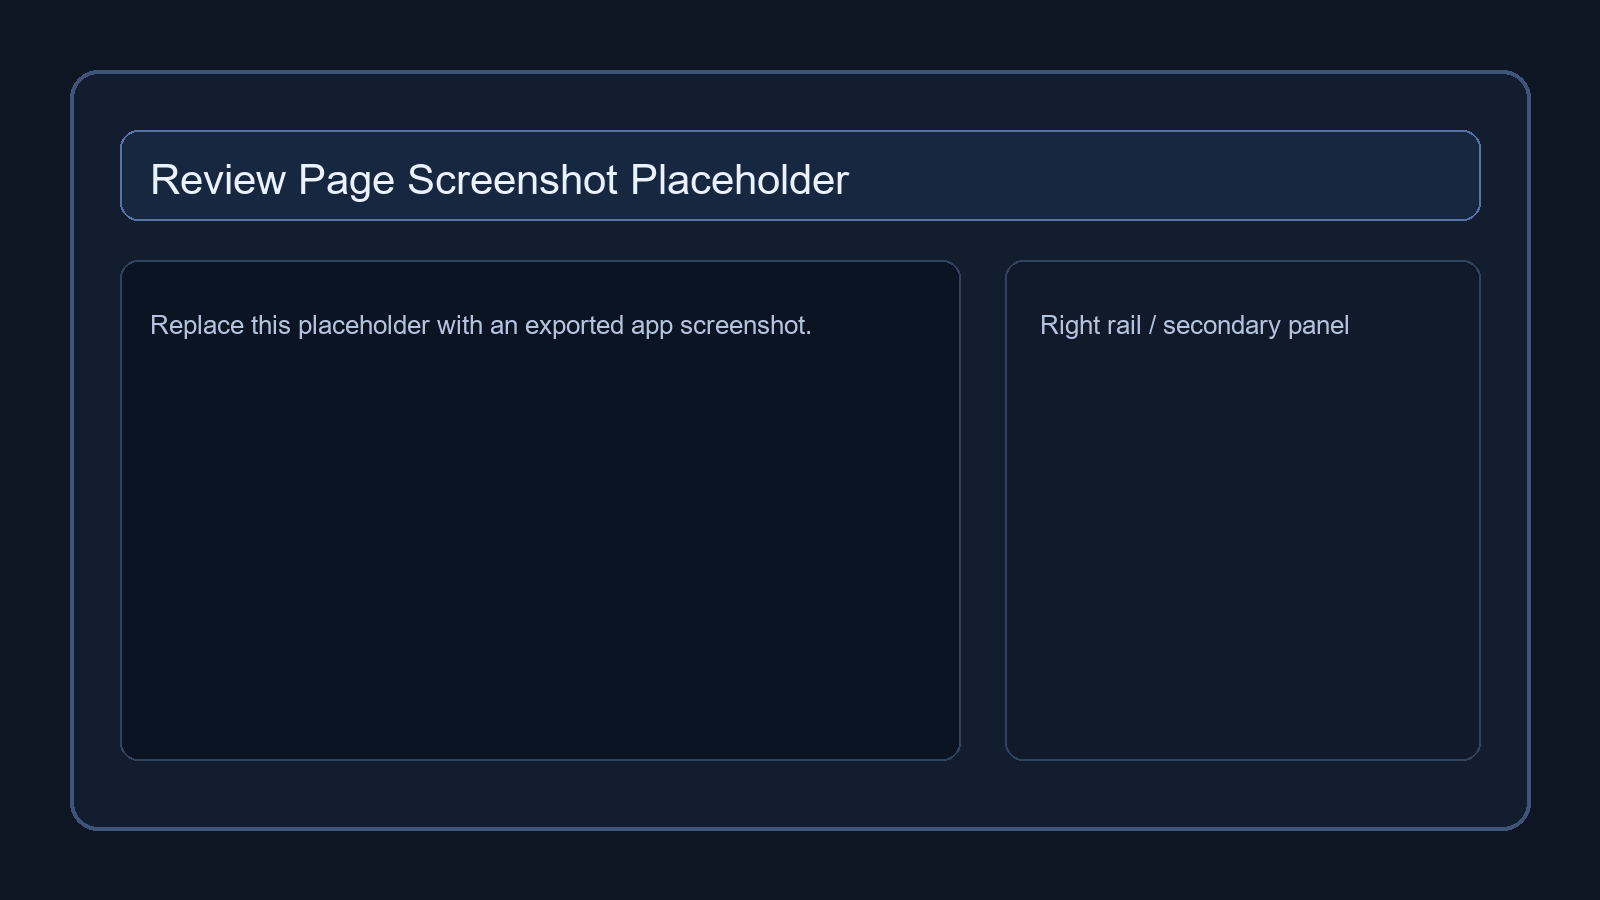
\includegraphics[width=\textwidth, height=5.5cm, keepaspectratio]{screenshot_review.png}

\column{0.44\textwidth}
\textbf{Annotated elements}
\begin{enumerate}
  \item \textbf{Property banner} — name, location, Expedia rating
  \item \textbf{Review text area} — monitored live for topic coverage
  \item \textbf{TWTK panel} (right column):
    \begin{itemize}
      \item GPT-4o-mini intro sentence per property
      \item Per-topic badges: Travelers asking /
            Mixed reviews / Not documented
    \end{itemize}
  \item \textbf{``Why am I seeing this?''} expander — transparency
  \item \textbf{Post review} primary action button
\end{enumerate}
\end{columns}
\end{frame}


\begin{frame}{Product Demo: Feature 2 --- Browse Page}
\begin{columns}[T]
\column{0.52\textwidth}
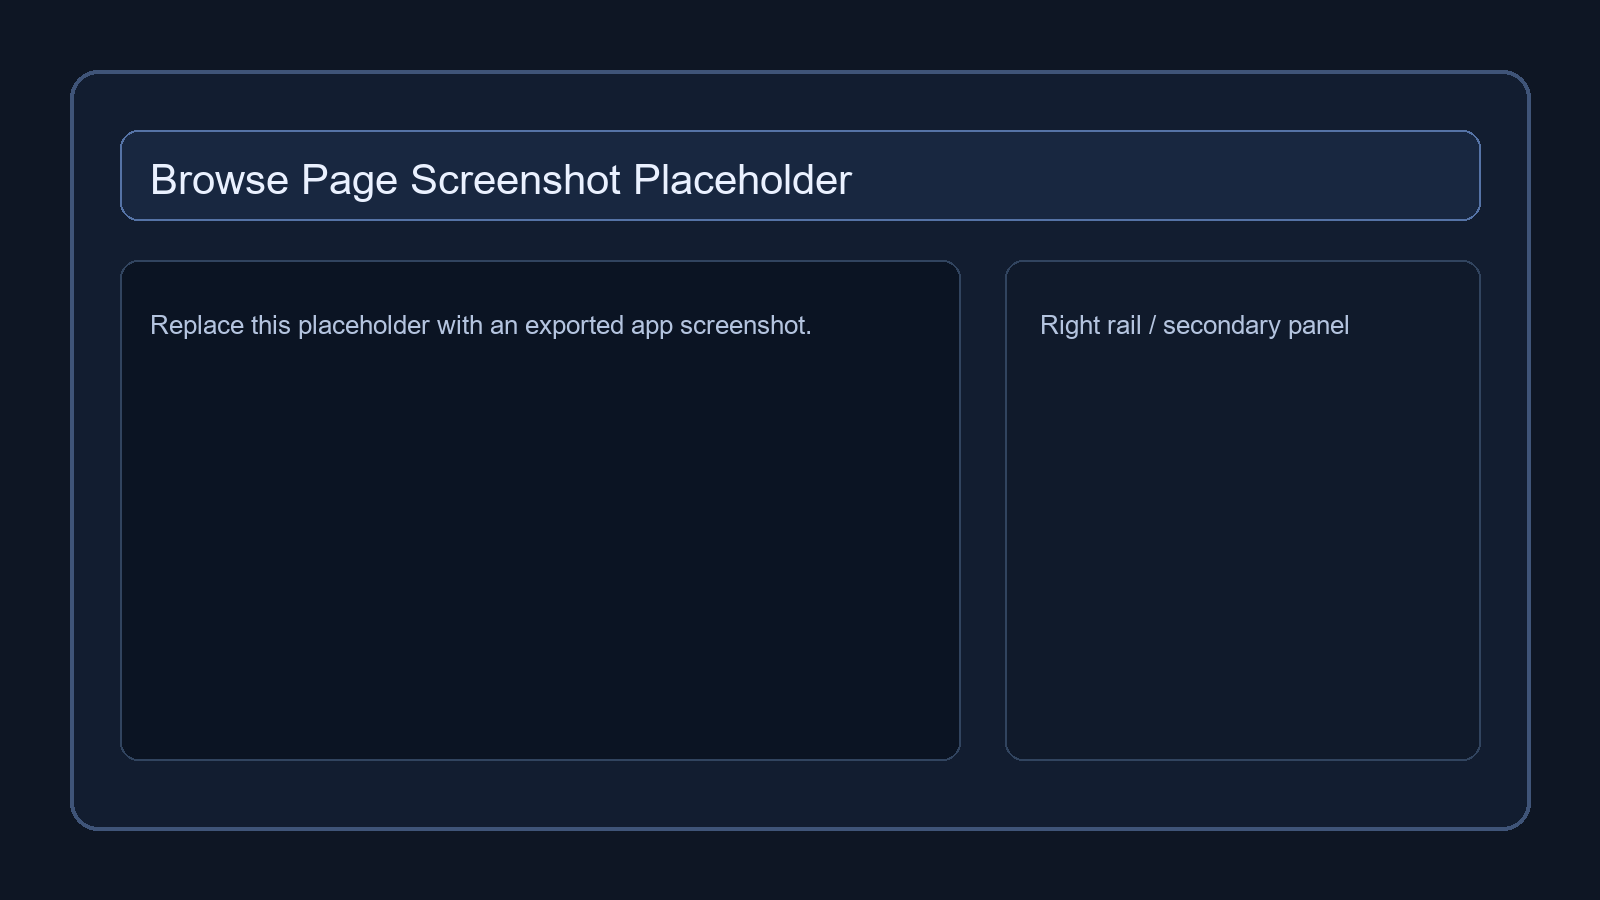
\includegraphics[width=\textwidth, height=5.5cm, keepaspectratio]{screenshot_browse.png}

\column{0.44\textwidth}
\textbf{Annotated elements}
\begin{enumerate}
  \item \textbf{Review cards} — dark surface cards with
        \textit{Read more $\downarrow$} toggle for long reviews
  \item \textbf{Rating badge} — overall score / 5
  \item \textbf{SNSAS form:}
    \begin{itemize}
      \item Free-text input
      \item Submit: embed \arrow\ classify \arrow\ save to CSV
      \item Text area clears via counter-keyed widget
    \end{itemize}
  \item Question count + Wipe button for demo resets
  \item Data written here feeds directly into the demand
        multiplier on the reviewer side
\end{enumerate}
\end{columns}
\end{frame}


% ════════════════════════════════════════════════════
\section{Summary}
% ════════════════════════════════════════════════════

\begin{frame}{Technical Summary}
\begin{columns}[T]
\column{0.48\textwidth}
\textbf{Stack}
\begin{itemize}
  \item Frontend / hosting: Streamlit (Python)
  \item Embeddings: \texttt{text-embedding-3-small}
  \item Language model: \texttt{gpt-4o-mini}
  \item Sentiment: VADER (local, $<$1ms/text)
  \item Data: Pandas / NumPy / CSV
  \item Caching: \texttt{@st.cache\_data} / \texttt{cache\_resource}
\end{itemize}

\medskip
\textbf{Key parameters}
\begin{itemize}
  \item $\theta_r = 0.40$ — topic relevance threshold
  \item $\theta_g = 0.15$ — coverage gap threshold
  \item $\theta_c = 0.38$ — contested sentiment std dev
  \item $\tau = 180$ days — decay half-life
  \item $N = 40$ — max reviews embedded
  \item $\beta_d = 3.0$ — demand sensitivity
  \item $k = 3$ — max TWTK topics shown
\end{itemize}

\column{0.48\textwidth}
\textbf{Information flows}
\begin{enumerate}
  \item Corpus \arrow\ embeddings \arrow\ coverage scores
  \item Corpus \arrow\ VADER \arrow\ contested flags
  \item Corpus + property desc \arrow\ LLM \arrow\ unique topics
  \item SNSAS questions \arrow\ classifier \arrow\ demand scores
  \item All signals \arrow\ scorer \arrow\ TWTK top-3
  \item Reviewer text \arrow\ per-sentence embeddings \arrow\ live feedback
  \item Submitted review \arrow\ LLM \arrow\ per-topic insights on thank-you page
\end{enumerate}
\end{columns}
\end{frame}

\end{document}
